\documentclass[ignorenonframetext,]{beamer}
\setbeamertemplate{caption}[numbered]
\setbeamertemplate{caption label separator}{: }
\setbeamercolor{caption name}{fg=normal text.fg}
\beamertemplatenavigationsymbolsempty
\usepackage{lmodern}
\usepackage{amssymb,amsmath}
\usepackage{ifxetex,ifluatex}
\usepackage{fixltx2e} % provides \textsubscript

\usetheme{CambridgeUS}
\definecolor{UBCblue}{rgb}{0.04706, 0.13725, 0.26667}
\definecolor{UBCgray}{rgb}{0.3686, 0.5255, 0.6235}
\colorlet{verylightgray}{gray!10}
\setbeamercolor{palette primary}{bg=UBCblue,fg=white}
\setbeamercolor{palette secondary}{bg=darkgray,fg=white}
\setbeamercolor{palette tertiary}{bg=UBCblue,fg=white}
\setbeamercolor{palette quaternary}{bg=UBCblue,fg=white}
\setbeamercolor{structure}{fg=UBCblue} % itemize, enumerate, etc
\setbeamercolor{section in toc}{fg=UBCblue} % TOC sections
\setbeamercolor{subsection in head/foot}{bg=darkgray,fg=white}
\setbeamercolor{frametitle}{fg=UBCblue}
\setbeamercolor{title}{fg=UBCblue, bg=verylightgray}
\setbeamertemplate{itemize items}{\color{UBCblue}$\blacktriangleright$}


\ifnum 0\ifxetex 1\fi\ifluatex 1\fi=0 % if pdftex
\usepackage[T1]{fontenc}
\usepackage[utf8]{inputenc}
\else % if luatex or xelatex
\ifxetex
\usepackage{mathspec}
\else
\usepackage{fontspec}
\fi
\defaultfontfeatures{Ligatures=TeX,Scale=MatchLowercase}
\fi
% use upquote if available, for straight quotes in verbatim environments
\IfFileExists{upquote.sty}{\usepackage{upquote}}{}
% use microtype if available
\IfFileExists{microtype.sty}{%
	\usepackage{microtype}
	\UseMicrotypeSet[protrusion]{basicmath} % disable protrusion for tt fonts
}{}
\newif\ifbibliography
\hypersetup{
	pdfauthor={UCSD},
	pdfborder={0 0 0},
	breaklinks=true}
\urlstyle{same}  % don't use monospace font for urls
\usepackage{color}
\usepackage{fancyvrb}
\newcommand{\VerbBar}{|}
\newcommand{\VERB}{\Verb[commandchars=\\\{\}]}
\DefineVerbatimEnvironment{Highlighting}{Verbatim}{commandchars=\\\{\}}
% Add ',fontsize=\small' for more characters per line
\usepackage{framed}
\definecolor{shadecolor}{RGB}{248,248,248}
\newenvironment{Shaded}{\begin{snugshade}}{\end{snugshade}}
\newcommand{\KeywordTok}[1]{\textcolor[rgb]{0.13,0.29,0.53}{\textbf{#1}}}
\newcommand{\DataTypeTok}[1]{\textcolor[rgb]{0.13,0.29,0.53}{#1}}
\newcommand{\DecValTok}[1]{\textcolor[rgb]{0.00,0.00,0.81}{#1}}
\newcommand{\BaseNTok}[1]{\textcolor[rgb]{0.00,0.00,0.81}{#1}}
\newcommand{\FloatTok}[1]{\textcolor[rgb]{0.00,0.00,0.81}{#1}}
\newcommand{\ConstantTok}[1]{\textcolor[rgb]{0.00,0.00,0.00}{#1}}
\newcommand{\CharTok}[1]{\textcolor[rgb]{0.31,0.60,0.02}{#1}}
\newcommand{\SpecialCharTok}[1]{\textcolor[rgb]{0.00,0.00,0.00}{#1}}
\newcommand{\StringTok}[1]{\textcolor[rgb]{0.31,0.60,0.02}{#1}}
\newcommand{\VerbatimStringTok}[1]{\textcolor[rgb]{0.31,0.60,0.02}{#1}}
\newcommand{\SpecialStringTok}[1]{\textcolor[rgb]{0.31,0.60,0.02}{#1}}
\newcommand{\ImportTok}[1]{#1}
\newcommand{\CommentTok}[1]{\textcolor[rgb]{0.56,0.35,0.01}{\textit{#1}}}
\newcommand{\DocumentationTok}[1]{\textcolor[rgb]{0.56,0.35,0.01}{\textbf{\textit{#1}}}}
\newcommand{\AnnotationTok}[1]{\textcolor[rgb]{0.56,0.35,0.01}{\textbf{\textit{#1}}}}
\newcommand{\CommentVarTok}[1]{\textcolor[rgb]{0.56,0.35,0.01}{\textbf{\textit{#1}}}}
\newcommand{\OtherTok}[1]{\textcolor[rgb]{0.56,0.35,0.01}{#1}}
\newcommand{\FunctionTok}[1]{\textcolor[rgb]{0.00,0.00,0.00}{#1}}
\newcommand{\VariableTok}[1]{\textcolor[rgb]{0.00,0.00,0.00}{#1}}
\newcommand{\ControlFlowTok}[1]{\textcolor[rgb]{0.13,0.29,0.53}{\textbf{#1}}}
\newcommand{\OperatorTok}[1]{\textcolor[rgb]{0.81,0.36,0.00}{\textbf{#1}}}
\newcommand{\BuiltInTok}[1]{#1}
\newcommand{\ExtensionTok}[1]{#1}
\newcommand{\PreprocessorTok}[1]{\textcolor[rgb]{0.56,0.35,0.01}{\textit{#1}}}
\newcommand{\AttributeTok}[1]{\textcolor[rgb]{0.77,0.63,0.00}{#1}}
\newcommand{\RegionMarkerTok}[1]{#1}
\newcommand{\InformationTok}[1]{\textcolor[rgb]{0.56,0.35,0.01}{\textbf{\textit{#1}}}}
\newcommand{\WarningTok}[1]{\textcolor[rgb]{0.56,0.35,0.01}{\textbf{\textit{#1}}}}
\newcommand{\AlertTok}[1]{\textcolor[rgb]{0.94,0.16,0.16}{#1}}
\newcommand{\ErrorTok}[1]{\textcolor[rgb]{0.64,0.00,0.00}{\textbf{#1}}}
\newcommand{\NormalTok}[1]{#1}
\usepackage{graphicx,grffile}
\makeatletter
\def\maxwidth{\ifdim\Gin@nat@width>\linewidth\linewidth\else\Gin@nat@width\fi}
\def\maxheight{\ifdim\Gin@nat@height>\textheight0.8\textheight\else\Gin@nat@height\fi}
\makeatother
% Scale images if necessary, so that they will not overflow the page
% margins by default, and it is still possible to overwrite the defaults
% using explicit options in \includegraphics[width, height, ...]{}
\setkeys{Gin}{width=\maxwidth,height=\maxheight,keepaspectratio}

% Prevent slide breaks in the middle of a paragraph:
\widowpenalties 1 10000
\raggedbottom

\AtBeginPart{
	\let\insertpartnumber\relax
	\let\partname\relax
	\frame{\partpage}
}
\AtBeginSection{
	\ifbibliography
	\else
	\let\insertsectionnumber\relax
	\let\sectionname\relax
	\frame{\sectionpage}
	\fi
}
\AtBeginSubsection{
	\let\insertsubsectionnumber\relax
	\let\subsectionname\relax
	\frame{\subsectionpage}
}

\setlength{\parindent}{0pt}
\setlength{\parskip}{6pt plus 2pt minus 1pt}
\setlength{\emergencystretch}{3em}  % prevent overfull lines
\providecommand{\tightlist}{%
	\setlength{\itemsep}{0pt}\setlength{\parskip}{0pt}}
\setcounter{secnumdepth}{0}


\title[Class 11]{Introduction to Social Data Analytics\\
	Week 6: Class 11}
\author{Arushi Kaushik}
\institute[UCSD]{arkaushi@ucsd.edu}
\date[Week6]{}


\begin{document}
\frame{\titlepage}

\begin{frame}{Today: Introduction to \texttt{R} and \texttt{RStudio}}

By the end of today's lecture, you should be able to:

\begin{itemize}
\tightlist
\item
  Locate and identify the essential parts of the RStudio interface
\item
  Create, edit, and save .R and .RData files
\item
  Generate objects and differentiate between datasets, numbers, strings,
  and functions
\end{itemize}

\end{frame}

\begin{frame}[fragile]{\texttt{RStudio} Interface}

\begin{figure}
\centering
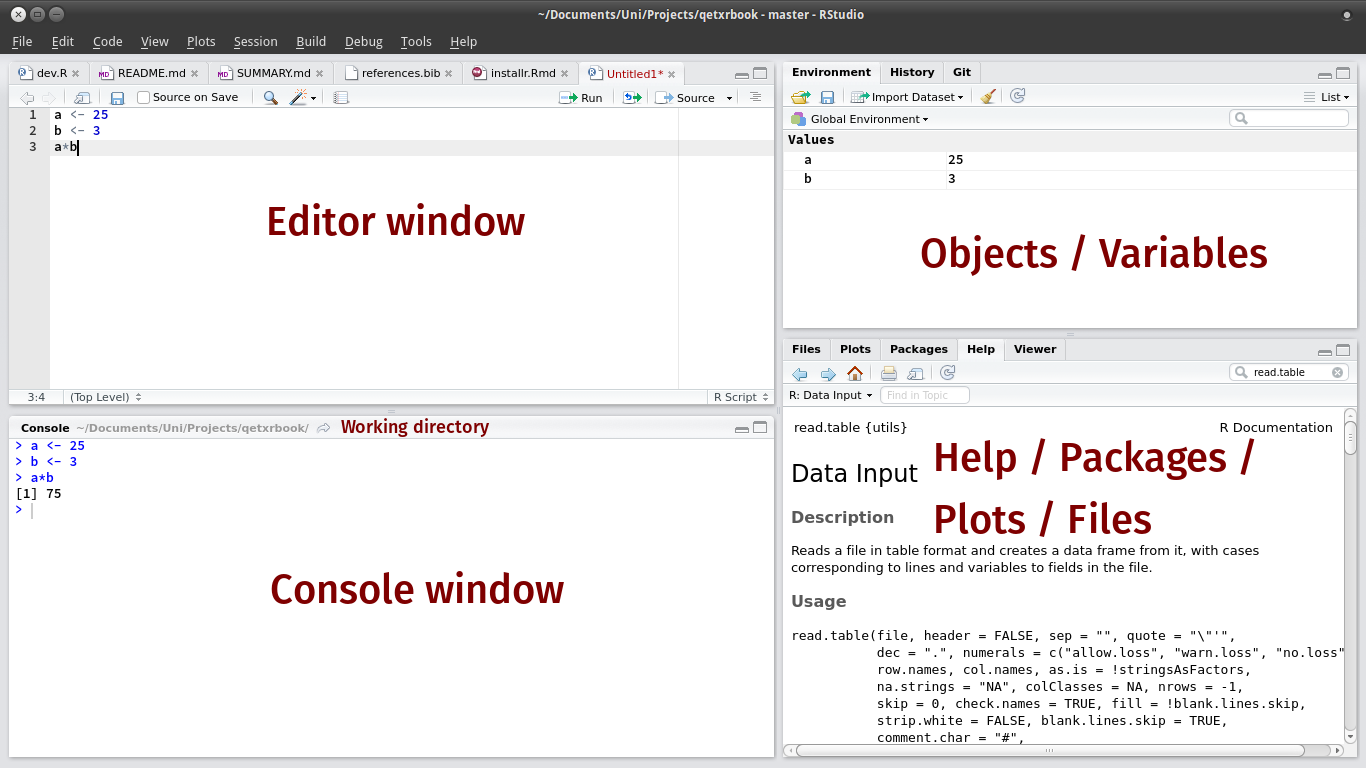
\includegraphics{rstudio.png}
\caption{\texttt{RStudio} Interface}
\end{figure}

\end{frame}

\begin{frame}[fragile]{Arithmetic Operations}

\texttt{R} can be used as a calculator:

\begin{Shaded}
\begin{Highlighting}[]
\DecValTok{5} \OperatorTok{+}\StringTok{ }\DecValTok{3}
\end{Highlighting}
\end{Shaded}

\begin{verbatim}
## [1] 8
\end{verbatim}

\begin{Shaded}
\begin{Highlighting}[]
\DecValTok{5} \OperatorTok{/}\StringTok{ }\DecValTok{3}
\end{Highlighting}
\end{Shaded}

\begin{verbatim}
## [1] 1.666667
\end{verbatim}

\begin{Shaded}
\begin{Highlighting}[]
\DecValTok{5} \OperatorTok{^}\StringTok{ }\DecValTok{3}
\end{Highlighting}
\end{Shaded}

\begin{verbatim}
## [1] 125
\end{verbatim}

\begin{itemize}
\tightlist
\item
  The {[}1{]} is telling you the row number.
\end{itemize}

\end{frame}

\begin{frame}[fragile]{\texttt{R} is an ``object-oriented'' programming
language}

\emph{Objects}, any pieces of information stored by \texttt{R}, can be:

\begin{itemize}
\tightlist
\item
  A dataset (e.g.~resume)
\item
  A subset of a dataset (e.g.~just the even observations of resume)
\item
  A number (e.g. \(2\pi + 1\))
\item
  A text string (e.g. ``UCSD is awesome'')
\item
  A function (e.g.~a function that takes in \(x\) and gives you
  \(x^2 + 8\))
\end{itemize}

\end{frame}

\begin{frame}[fragile]{Creating objects}

\texttt{R} can store \emph{objects} with a name of our choice. Use
\texttt{\textless{}-} as an assignment operator for objects.

\begin{Shaded}
\begin{Highlighting}[]
\NormalTok{object_}\DecValTok{1}\NormalTok{ <-}\StringTok{ }\DecValTok{5} \OperatorTok{+}\StringTok{ }\DecValTok{3}
\NormalTok{object_}\DecValTok{1}
\end{Highlighting}
\end{Shaded}

\begin{verbatim}
## [1] 8
\end{verbatim}

If we assign a new value to the same object name, then we will overwrite
this object (so be careful when doing so!)

\begin{Shaded}
\begin{Highlighting}[]
\NormalTok{object_}\DecValTok{1}\NormalTok{ <-}\StringTok{ }\DecValTok{5} \OperatorTok{-}\StringTok{ }\DecValTok{3}
\NormalTok{object_}\DecValTok{1}
\end{Highlighting}
\end{Shaded}

\begin{verbatim}
## [1] 2
\end{verbatim}

\end{frame}

\begin{frame}[fragile]{Objects (cont.)}

\texttt{R} can also represent other types of values as objects, such as
strings of characters:

\begin{Shaded}
\begin{Highlighting}[]
\NormalTok{MySchool <-}\StringTok{ "UCSD"}
\NormalTok{MySchool}
\end{Highlighting}
\end{Shaded}

\begin{verbatim}
## [1] "UCSD"
\end{verbatim}

\end{frame}

\begin{frame}[fragile]{A \emph{vector} represents a collection of
information stored in a specific order}

We use the function \texttt{c()}, which stands for ``concatenate,'' to
enter a data vector (with commas separating elements of the vector):

\begin{Shaded}
\begin{Highlighting}[]
\NormalTok{vector.}\DecValTok{1}\NormalTok{ <-}\StringTok{ }\KeywordTok{c}\NormalTok{(}\DecValTok{93}\NormalTok{, }\DecValTok{92}\NormalTok{, }\DecValTok{83}\NormalTok{, }\DecValTok{99}\NormalTok{, }\DecValTok{96}\NormalTok{, }\DecValTok{97}\NormalTok{)}
\NormalTok{vector.}\DecValTok{1}
\end{Highlighting}
\end{Shaded}

\begin{verbatim}
## [1] 93 92 83 99 96 97
\end{verbatim}

\begin{itemize}
\tightlist
\item
  Note: when creating a vector, R creates column vectors
  \((n \times 1)\)
\end{itemize}

\end{frame}

\begin{frame}[fragile]{Vectors (cont.)}

To access specific elements of a vector, we use square brackets\\
\texttt{{[}\ {]}}. This is called \emph{indexing}:

\begin{Shaded}
\begin{Highlighting}[]
\NormalTok{vector.}\DecValTok{1}\NormalTok{[}\DecValTok{2}\NormalTok{]}
\end{Highlighting}
\end{Shaded}

\begin{verbatim}
## [1] 92
\end{verbatim}

\begin{Shaded}
\begin{Highlighting}[]
\NormalTok{vector.}\DecValTok{1}\NormalTok{[}\KeywordTok{c}\NormalTok{(}\DecValTok{2}\NormalTok{, }\DecValTok{4}\NormalTok{)]}
\end{Highlighting}
\end{Shaded}

\begin{verbatim}
## [1] 92 99
\end{verbatim}

\begin{Shaded}
\begin{Highlighting}[]
\NormalTok{vector.}\DecValTok{1}\NormalTok{[}\OperatorTok{-}\DecValTok{4}\NormalTok{]}
\end{Highlighting}
\end{Shaded}

\begin{verbatim}
## [1] 93 92 83 96 97
\end{verbatim}

\end{frame}

\begin{frame}[fragile]{Vectors (cont.)}

Since each element of this vector is a numeric value, we can apply
arithmetic operations to it:

\begin{Shaded}
\begin{Highlighting}[]
\NormalTok{vector.}\DecValTok{1} \OperatorTok{*}\StringTok{ }\DecValTok{1000}
\end{Highlighting}
\end{Shaded}

\begin{verbatim}
## [1] 93000 92000 83000 99000 96000 97000
\end{verbatim}

\end{frame}

\begin{frame}[fragile]{Element-corresponding operations with vectors}

\begin{Shaded}
\begin{Highlighting}[]
\NormalTok{vec1 <-}\StringTok{ }\KeywordTok{c}\NormalTok{(}\DecValTok{1}\NormalTok{, }\DecValTok{2}\NormalTok{, }\DecValTok{3}\NormalTok{); vec2 <-}\StringTok{ }\KeywordTok{c}\NormalTok{(}\DecValTok{3}\NormalTok{, }\DecValTok{3}\NormalTok{, }\DecValTok{3}\NormalTok{)}
\NormalTok{vec1 }\OperatorTok{+}\StringTok{ }\NormalTok{vec2}
\end{Highlighting}
\end{Shaded}

\begin{verbatim}
## [1] 4 5 6
\end{verbatim}

\begin{Shaded}
\begin{Highlighting}[]
\NormalTok{vec1 }\OperatorTok{*}\StringTok{ }\NormalTok{vec2}
\end{Highlighting}
\end{Shaded}

\begin{verbatim}
## [1] 3 6 9
\end{verbatim}

\begin{Shaded}
\begin{Highlighting}[]
\NormalTok{vec1 }\OperatorTok{/}\StringTok{ }\NormalTok{vec2}
\end{Highlighting}
\end{Shaded}

\begin{verbatim}
## [1] 0.3333333 0.6666667 1.0000000
\end{verbatim}

\end{frame}

\begin{frame}[fragile]{Functions}

A \emph{function} takes input object(s) and returns an output object. In
\texttt{R}, a function generally runs as \texttt{funcname(input)}. Some
basic functions useful for summarizing data include:

\begin{itemize}
\tightlist
\item
  \texttt{length()}: length of a vector (number of elements)
\item
  \texttt{min()}: minimum value
\item
  \texttt{max()}: maximum value
\item
  \texttt{range()}: range of data
\item
  \texttt{mean()}: mean
\item
  \texttt{sum()}: sum
\end{itemize}

Try these with \texttt{vector.1}

\end{frame}

\begin{frame}[fragile]{Functions (cont.)}

\begin{Shaded}
\begin{Highlighting}[]
\KeywordTok{length}\NormalTok{(vector.}\DecValTok{1}\NormalTok{)}
\end{Highlighting}
\end{Shaded}

\begin{verbatim}
## [1] 6
\end{verbatim}

\begin{Shaded}
\begin{Highlighting}[]
\KeywordTok{min}\NormalTok{(vector.}\DecValTok{1}\NormalTok{)}
\end{Highlighting}
\end{Shaded}

\begin{verbatim}
## [1] 83
\end{verbatim}

\begin{Shaded}
\begin{Highlighting}[]
\KeywordTok{max}\NormalTok{(vector.}\DecValTok{1}\NormalTok{)}
\end{Highlighting}
\end{Shaded}

\begin{verbatim}
## [1] 99
\end{verbatim}

\end{frame}

\begin{frame}[fragile]{Functions (cont.)}

\begin{Shaded}
\begin{Highlighting}[]
\KeywordTok{range}\NormalTok{(vector.}\DecValTok{1}\NormalTok{)}
\end{Highlighting}
\end{Shaded}

\begin{verbatim}
## [1] 83 99
\end{verbatim}

\begin{Shaded}
\begin{Highlighting}[]
\KeywordTok{mean}\NormalTok{(vector.}\DecValTok{1}\NormalTok{)}
\end{Highlighting}
\end{Shaded}

\begin{verbatim}
## [1] 93.33333
\end{verbatim}

\begin{Shaded}
\begin{Highlighting}[]
\KeywordTok{sum}\NormalTok{(vector.}\DecValTok{1}\NormalTok{)}
\end{Highlighting}
\end{Shaded}

\begin{verbatim}
## [1] 560
\end{verbatim}

\end{frame}

\begin{frame}[fragile]{Like Stata, we need to specify a working
directory in \texttt{R}}

\begin{itemize}
\tightlist
\item
  Use the function \texttt{setwd()} to change the working directory
\end{itemize}

\begin{Shaded}
\begin{Highlighting}[]
\KeywordTok{setwd}\NormalTok{(}\StringTok{"path"}\NormalTok{)}
\end{Highlighting}
\end{Shaded}

\begin{itemize}
\tightlist
\item
  Use the function \texttt{getwd()} to display the current working
  directory.
\end{itemize}

\begin{Shaded}
\begin{Highlighting}[]
\KeywordTok{getwd}\NormalTok{()}
\end{Highlighting}
\end{Shaded}

\texttt{\#\#\ {[}1{]}\ path}

\end{frame}

\begin{frame}[fragile]{Loading data from your working directory}

\begin{itemize}
\tightlist
\item
  For \emph{CSV} files:
\end{itemize}

\begin{Shaded}
\begin{Highlighting}[]
\NormalTok{resume <-}\StringTok{ }\KeywordTok{read.csv}\NormalTok{(}\StringTok{"resume.csv"}\NormalTok{)}
\end{Highlighting}
\end{Shaded}

\begin{itemize}
\tightlist
\item
  For \emph{RData} files:
\end{itemize}

\begin{Shaded}
\begin{Highlighting}[]
\NormalTok{resume <-}\StringTok{ }\KeywordTok{load}\NormalTok{(}\StringTok{"resume.RData"}\NormalTok{)}
\end{Highlighting}
\end{Shaded}

\end{frame}

\begin{frame}[fragile]{Data Frames}

A \emph{data frame} is a collection of vectors, but we can think of it
like an Excel spreadsheet. Useful functions for data frames include:

\begin{itemize}
\tightlist
\item
  \texttt{names()}: return a vector of variable names
\item
  \texttt{nrow()}: return the number of rows
\item
  \texttt{ncol()}: return the number of columns
\item
  \texttt{dim()}: combine \texttt{ncol()} and \texttt{nrow()} into a
  vector
\item
  \texttt{summary()}: produce a summary
\item
  \texttt{head()}: displays the first six observations
\item
  \texttt{tail()}: displays the last six observations
\end{itemize}

Load \texttt{resume.csv}, assign it to an object called \texttt{resume},
and try the above functions on this newly created data frame.

\end{frame}

\begin{frame}[fragile]{Data Frames (cont.)}

\begin{Shaded}
\begin{Highlighting}[]
\KeywordTok{names}\NormalTok{(resume)}
\end{Highlighting}
\end{Shaded}

\begin{verbatim}
## [1] "X"         "firstname" "sex"       "race"      "call"
\end{verbatim}

\begin{Shaded}
\begin{Highlighting}[]
\KeywordTok{nrow}\NormalTok{(resume)}
\end{Highlighting}
\end{Shaded}

\begin{verbatim}
## [1] 4870
\end{verbatim}

\begin{Shaded}
\begin{Highlighting}[]
\KeywordTok{ncol}\NormalTok{(resume)}
\end{Highlighting}
\end{Shaded}

\begin{verbatim}
## [1] 5
\end{verbatim}

\end{frame}

\begin{frame}[fragile]{Data Frames (cont.)}

\begin{Shaded}
\begin{Highlighting}[]
\KeywordTok{dim}\NormalTok{(resume)}
\end{Highlighting}
\end{Shaded}

\begin{verbatim}
## [1] 4870    5
\end{verbatim}

\begin{Shaded}
\begin{Highlighting}[]
\KeywordTok{summary}\NormalTok{(resume)}
\end{Highlighting}
\end{Shaded}

\begin{verbatim}
##        X          firstname        sex          race     
##  Min.   :   1   Tamika : 256   female:3746   black:2435  
##  1st Qu.:1218   Anne   : 242   male  :1124   white:2435  
##  Median :2436   Allison: 232                             
##  Mean   :2436   Latonya: 230                             
##  3rd Qu.:3653   Emily  : 227                             
##  Max.   :4870   Latoya : 226                             
##                 (Other):3457                             
##       call        
##  Min.   :0.00000  
##  1st Qu.:0.00000  
##  Median :0.00000  
##  Mean   :0.08049  
##  3rd Qu.:0.00000  
##  Max.   :1.00000  
## 
\end{verbatim}

\end{frame}

\begin{frame}[fragile]{Data Frames (cont.)}

\begin{Shaded}
\begin{Highlighting}[]
\KeywordTok{head}\NormalTok{(resume)}
\end{Highlighting}
\end{Shaded}

\begin{verbatim}
##   X firstname    sex  race call
## 1 1   Allison female white    0
## 2 2   Kristen female white    0
## 3 3   Lakisha female black    0
## 4 4   Latonya female black    0
## 5 5    Carrie female white    0
## 6 6       Jay   male white    0
\end{verbatim}

\begin{Shaded}
\begin{Highlighting}[]
\KeywordTok{tail}\NormalTok{(resume)}
\end{Highlighting}
\end{Shaded}

\begin{verbatim}
##         X firstname    sex  race call
## 4865 4865   Lakisha female black    0
## 4866 4866    Tamika female black    0
## 4867 4867     Ebony female black    0
## 4868 4868       Jay   male white    0
## 4869 4869   Latonya female black    0
## 4870 4870    Laurie female white    0
\end{verbatim}

\end{frame}

\begin{frame}[fragile]{Data Frames: using {[}{]}}

We can retrieve specified observations and variables using brackets
\texttt{{[}\ {]}} with a comma in the form
\texttt{{[}rows,\ columns{]}}:

\begin{Shaded}
\begin{Highlighting}[]
\NormalTok{resume[}\DecValTok{1}\OperatorTok{:}\DecValTok{3}\NormalTok{, }\StringTok{"firstname"}\NormalTok{]}
\end{Highlighting}
\end{Shaded}

\begin{verbatim}
## [1] Allison Kristen Lakisha
## 36 Levels: Aisha Allison Anne Brad Brendan Brett Carrie Darnell ... Tyrone
\end{verbatim}

\begin{Shaded}
\begin{Highlighting}[]
\NormalTok{resume[}\DecValTok{1}\OperatorTok{:}\DecValTok{3}\NormalTok{, }\DecValTok{2}\NormalTok{]}
\end{Highlighting}
\end{Shaded}

\begin{verbatim}
## [1] Allison Kristen Lakisha
## 36 Levels: Aisha Allison Anne Brad Brendan Brett Carrie Darnell ... Tyrone
\end{verbatim}

Observe that ``firstname'' is the second variable in the ``resume'' data
frame.

\end{frame}

\begin{frame}[fragile]{Data Frames: using \$}

The \texttt{\$} operator is another way to access variables from a data
frame:

\begin{Shaded}
\begin{Highlighting}[]
\KeywordTok{head}\NormalTok{(resume}\OperatorTok{$}\NormalTok{firstname, }\DecValTok{3}\NormalTok{)}
\end{Highlighting}
\end{Shaded}

\begin{verbatim}
## [1] Allison Kristen Lakisha
## 36 Levels: Aisha Allison Anne Brad Brendan Brett Carrie Darnell ... Tyrone
\end{verbatim}

Note: the ``3'' after the comma specifies how many observations to
display.

\end{frame}

\begin{frame}[fragile]{Saving Objects}

When you quit \texttt{RStudio}, you will be asked whether you would like
to save the workspace. You should answer \emph{no} to this in general:
we only want to save what we want!

\begin{itemize}
\tightlist
\item
  To export \emph{CSV}:
\end{itemize}

\begin{Shaded}
\begin{Highlighting}[]
\KeywordTok{write.csv}\NormalTok{(resume, }\DataTypeTok{file =} \StringTok{"resume.csv"}\NormalTok{)}
\end{Highlighting}
\end{Shaded}

\begin{itemize}
\tightlist
\item
  To export \emph{RData}:
\end{itemize}

\begin{Shaded}
\begin{Highlighting}[]
\KeywordTok{save}\NormalTok{(resume, }\DataTypeTok{file =} \StringTok{"resume.RData"}\NormalTok{)}
\end{Highlighting}
\end{Shaded}

Go ahead and export your data frame as RData.

\end{frame}

\begin{frame}[fragile]{Here are the commands/operators we covered
today:}

\begin{itemize}
\tightlist
\item
  \texttt{\textless{}-}
\item
  \texttt{c()}
\item
  \texttt{vector{[}{]}}
\item
  \texttt{length(),\ min(),\ max(),\ range(),\ mean(),\ sum()}
\item
  \texttt{head(),\ tail()}
\item
  \texttt{setwd(),\ getwd()}
\item
  \texttt{read.csv(),\ load()}
\item
  \texttt{names(),\ nrow(),\ ncol(),\ dim(),\ summary()}
\item
  \texttt{write.csv(),\ save()}
\item
  \texttt{\$}
\end{itemize}

\end{frame}

\end{document}
